% TODO: Talk about the changes we made after the first round of tutori
The team performed evaluations in person and over two days.  At the end of
the first day, there were a few issues that had been consistently pointed out
that were fairly straightforward to fix.  To help focus on evaluating the speed
of use of the system, the team opted to fix a few of these issues immediately
before the second round of tutoring. In addition to these changes, section \ref{sec:mock}
discusses slight alterations made to the databases after evaluation day 1.

\begin{figure}
  \caption{The tutor display prompt for a volunteer.} \label{fig:tutor_display}
  \centering
    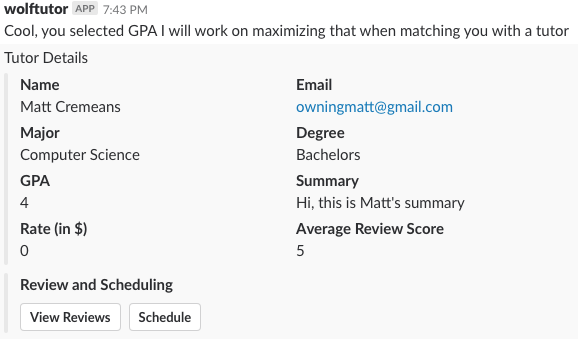
\includegraphics[width=0.5\textwidth]{tutor-display.png}
\end{figure}

% Fixed prompt to display rate as a currency
The first thing that was changed was a menu from the original system.  In the
original system, the tutor display had a "Rate'' section that was intended to
display that tutor's billing rate.  During our trials, testers consistently
mistook this for a rating, so the team made the decision to add the quantifier
added in figure \ref{fig:tutor_display} switch things out.

% Added average tutor score to tutor display
The team also decided to add one other menu item. During the initial
development, the team intended to add average tutor review score to the same
tutor display discussed above, but overlooked that simple enhancement at the
time.  This made it more difficult for students to actually run the tests,
though it was still possible through the use of the original ``review'' view.
This field is also visible in figure \ref{fig:tutor_display}.

% Fixed order of tutors display
The final major change made after the first round of tutoring was a bugfix.
During the first round of evaluations, the team realized that the tutors being
displayed were displaying out of order from what the team expected.  After
investigating, it was discovered that the suggestion algorithm was not
malfunctioning as originally thought, but that the Slack API used to send the
tutor suggestions to the users was delivering messages asynchronously, rather
than synchronously as had been thought during development and initial testing.
This was rectified by changing to a different interface that, while slower
because it performed a handshake with every message, delivered the messages in
the correct order.  

%%% Local Variables:
%%% mode: latex
%%% TeX-master: "../main"
%%% End:
